% Options for packages loaded elsewhere
\PassOptionsToPackage{unicode}{hyperref}
\PassOptionsToPackage{hyphens}{url}
\PassOptionsToPackage{dvipsnames,svgnames,x11names}{xcolor}
%
\documentclass[
  letterpaper,
  DIV=11,
  numbers=noendperiod]{scrartcl}

\usepackage{amsmath,amssymb}
\usepackage{iftex}
\ifPDFTeX
  \usepackage[T1]{fontenc}
  \usepackage[utf8]{inputenc}
  \usepackage{textcomp} % provide euro and other symbols
\else % if luatex or xetex
  \usepackage{unicode-math}
  \defaultfontfeatures{Scale=MatchLowercase}
  \defaultfontfeatures[\rmfamily]{Ligatures=TeX,Scale=1}
\fi
\usepackage{lmodern}
\ifPDFTeX\else  
    % xetex/luatex font selection
\fi
% Use upquote if available, for straight quotes in verbatim environments
\IfFileExists{upquote.sty}{\usepackage{upquote}}{}
\IfFileExists{microtype.sty}{% use microtype if available
  \usepackage[]{microtype}
  \UseMicrotypeSet[protrusion]{basicmath} % disable protrusion for tt fonts
}{}
\makeatletter
\@ifundefined{KOMAClassName}{% if non-KOMA class
  \IfFileExists{parskip.sty}{%
    \usepackage{parskip}
  }{% else
    \setlength{\parindent}{0pt}
    \setlength{\parskip}{6pt plus 2pt minus 1pt}}
}{% if KOMA class
  \KOMAoptions{parskip=half}}
\makeatother
\usepackage{xcolor}
\setlength{\emergencystretch}{3em} % prevent overfull lines
\setcounter{secnumdepth}{-\maxdimen} % remove section numbering
% Make \paragraph and \subparagraph free-standing
\makeatletter
\ifx\paragraph\undefined\else
  \let\oldparagraph\paragraph
  \renewcommand{\paragraph}{
    \@ifstar
      \xxxParagraphStar
      \xxxParagraphNoStar
  }
  \newcommand{\xxxParagraphStar}[1]{\oldparagraph*{#1}\mbox{}}
  \newcommand{\xxxParagraphNoStar}[1]{\oldparagraph{#1}\mbox{}}
\fi
\ifx\subparagraph\undefined\else
  \let\oldsubparagraph\subparagraph
  \renewcommand{\subparagraph}{
    \@ifstar
      \xxxSubParagraphStar
      \xxxSubParagraphNoStar
  }
  \newcommand{\xxxSubParagraphStar}[1]{\oldsubparagraph*{#1}\mbox{}}
  \newcommand{\xxxSubParagraphNoStar}[1]{\oldsubparagraph{#1}\mbox{}}
\fi
\makeatother


\providecommand{\tightlist}{%
  \setlength{\itemsep}{0pt}\setlength{\parskip}{0pt}}\usepackage{longtable,booktabs,array}
\usepackage{calc} % for calculating minipage widths
% Correct order of tables after \paragraph or \subparagraph
\usepackage{etoolbox}
\makeatletter
\patchcmd\longtable{\par}{\if@noskipsec\mbox{}\fi\par}{}{}
\makeatother
% Allow footnotes in longtable head/foot
\IfFileExists{footnotehyper.sty}{\usepackage{footnotehyper}}{\usepackage{footnote}}
\makesavenoteenv{longtable}
\usepackage{graphicx}
\makeatletter
\def\maxwidth{\ifdim\Gin@nat@width>\linewidth\linewidth\else\Gin@nat@width\fi}
\def\maxheight{\ifdim\Gin@nat@height>\textheight\textheight\else\Gin@nat@height\fi}
\makeatother
% Scale images if necessary, so that they will not overflow the page
% margins by default, and it is still possible to overwrite the defaults
% using explicit options in \includegraphics[width, height, ...]{}
\setkeys{Gin}{width=\maxwidth,height=\maxheight,keepaspectratio}
% Set default figure placement to htbp
\makeatletter
\def\fps@figure{htbp}
\makeatother

\usepackage{booktabs}
\usepackage{longtable}
\usepackage{array}
\usepackage{multirow}
\usepackage{wrapfig}
\usepackage{float}
\usepackage{colortbl}
\usepackage{pdflscape}
\usepackage{tabu}
\usepackage{threeparttable}
\usepackage{threeparttablex}
\usepackage[normalem]{ulem}
\usepackage{makecell}
\usepackage{xcolor}
\usepackage{fvextra}
\DefineVerbatimEnvironment{Highlighting}{Verbatim}{breaklines,commandchars=\\\{\}}
 \DefineVerbatimEnvironment{OutputCode}{Verbatim}{breaklines,commandchars=\\\{\}}
\KOMAoption{captions}{tableheading}
\makeatletter
\@ifpackageloaded{caption}{}{\usepackage{caption}}
\AtBeginDocument{%
\ifdefined\contentsname
  \renewcommand*\contentsname{Table of contents}
\else
  \newcommand\contentsname{Table of contents}
\fi
\ifdefined\listfigurename
  \renewcommand*\listfigurename{List of Figures}
\else
  \newcommand\listfigurename{List of Figures}
\fi
\ifdefined\listtablename
  \renewcommand*\listtablename{List of Tables}
\else
  \newcommand\listtablename{List of Tables}
\fi
\ifdefined\figurename
  \renewcommand*\figurename{Figure}
\else
  \newcommand\figurename{Figure}
\fi
\ifdefined\tablename
  \renewcommand*\tablename{Table}
\else
  \newcommand\tablename{Table}
\fi
}
\@ifpackageloaded{float}{}{\usepackage{float}}
\floatstyle{ruled}
\@ifundefined{c@chapter}{\newfloat{codelisting}{h}{lop}}{\newfloat{codelisting}{h}{lop}[chapter]}
\floatname{codelisting}{Listing}
\newcommand*\listoflistings{\listof{codelisting}{List of Listings}}
\makeatother
\makeatletter
\makeatother
\makeatletter
\@ifpackageloaded{caption}{}{\usepackage{caption}}
\@ifpackageloaded{subcaption}{}{\usepackage{subcaption}}
\makeatother

\ifLuaTeX
  \usepackage{selnolig}  % disable illegal ligatures
\fi
\usepackage{bookmark}

\IfFileExists{xurl.sty}{\usepackage{xurl}}{} % add URL line breaks if available
\urlstyle{same} % disable monospaced font for URLs
\hypersetup{
  pdftitle={FPCP3},
  pdfauthor={Robin Tran},
  colorlinks=true,
  linkcolor={blue},
  filecolor={Maroon},
  citecolor={Blue},
  urlcolor={Blue},
  pdfcreator={LaTeX via pandoc}}


\title{FPCP3}
\author{Robin Tran}
\date{}

\begin{document}
\maketitle


\section{Introduction}\label{introduction}

This project explores customer behavior using a dataset with
demographic, transactional, and engagement features. There are two main
sections. In the first section, we implemented linear regression models
to predict each customer's average transaction value, comparing
different model specifications using 10-fold cross-validation. In the
second section, we used logistic regression to classify whether a
customer is at high churn risk based on selected predictors. The goal is
to understand what factors are associated with customer spending and
retention, and to evaluate model performance using appropriate
validation techniques.

\subsection{Variables of Interest}\label{variables-of-interest}

I will be considering 7 numerical variables and 12 categorical
variables. They are listed below along.

\begin{table}[!h]

\caption{Numerical Variables}
\centering
\fontsize{10}{12}\selectfont
\begin{tabular}[t]{l>{\raggedright\arraybackslash}p{10cm}}
\toprule
Variable & Description\\
\midrule
age & The age of the user, measured in years.\\
days\_since\_last\_login & The number of days since the user last logged into the website, measured in days.\\
avg\_time\_spent & The average amount of time the user spends per visit on the website, measured in minutes.\\
avg\_transaction\_value & The average value of transactions made by the user, measured in monetary units (currency).\\
avg\_frequency\_login\_days & The average number of days between the user's consecutive logins, measured in days.\\
points\_in\_wallet & The amount of loyalty or reward points currently available in the user's wallet, measured in points.\\
churn\_risk\_score & The churn risk score assigned to the user, ranging from 1 to 5, indicating the likelihood of the user leaving the service (higher scores indicate higher risk).\\
\bottomrule
\end{tabular}
\end{table}

\begin{table}[!h]

\caption{Categorical Variables}
\centering
\fontsize{10}{12}\selectfont
\begin{tabular}[t]{l>{\raggedright\arraybackslash}p{12cm}}
\toprule
Variable & Categories\\
\midrule
gender & F, M, Unknown\\
region\_category & Village, City, Town\\
membership\_category & Platinum Membership, Premium Membership, No Membership, Gold Membership, Silver Membership, Basic Membership\\
joined\_through\_referral & Yes, No\\
preferred\_offer\_types & Gift Vouchers/Coupons, Credit/Debit Card Offers, Without Offers\\
medium\_of\_operation & Desktop, Smartphone, Both\\
internet\_option & Wi-Fi, Mobile\_Data, Fiber\_Optic\\
used\_special\_discount & Yes, No\\
offer\_application\_preference & Yes, No\\
past\_complaint & Yes, No\\
complaint\_status & Not Applicable, Solved, Solved in Follow-up, Unsolved, No Information Available\\
feedback & Products always in Stock, Quality Customer Care, Poor Website, No reason specified, Poor Product Quality, Poor Customer Service, Too many ads, User Friendly Website, Reasonable Price\\
\bottomrule
\end{tabular}
\end{table}

\subsection{Observational Unit}\label{observational-unit}

Each row in the data set represents one individual customer who has
engaged with the platform and has at least one recorded purchase.

We also verified the categorical variables' types.

\section{Exploratory Data Analysis}\label{exploratory-data-analysis}

\subsection{Summaries}\label{summaries}

We included statistical summary for our numerical variables as below.

\begin{table}[!h]

\caption{Summary Statistics for Numerical Variables}
\centering
\fontsize{10}{12}\selectfont
\begin{tabular}[t]{lrrrrrrr}
\toprule
Variable & mean & median & sd & IQR & min & max & n\\
\midrule
age & 37.08 & 37.00 & 15.91 & 28.00 & 10.00 & 64.00 & 24853\\
days\_since\_last\_login & -42.61 & 12.00 & 230.18 & 8.00 & -999.00 & 26.00 & 24853\\
avg\_time\_spent & 244.14 & 162.37 & 398.10 & 295.65 & -2281.24 & 3040.41 & 24853\\
avg\_transaction\_value & 29321.54 & 27534.68 & 19499.51 & 26605.22 & 800.46 & 99914.05 & 24853\\
avg\_frequency\_login\_days & 15.97 & 16.00 & 9.23 & 14.00 & -43.65 & 73.06 & 24853\\
\addlinespace
points\_in\_wallet & 688.30 & 698.66 & 195.79 & 148.52 & -760.66 & 2069.07 & 24853\\
churn\_risk\_score & 3.61 & 4.00 & 1.18 & 2.00 & 1.00 & 5.00 & 24853\\
\bottomrule
\end{tabular}
\end{table}

We also included statistical summaries for some of our categorical
variables as below. The summaries are quite insightful. We observe
balanced classes in \texttt{gender}, but there might be some imbalances
in \texttt{membership\_category} and \texttt{region\_category}.

\begin{table}[!h]

\caption{Distribution of Gender}
\centering
\fontsize{10}{12}\selectfont
\begin{tabular}[t]{lrr}
\toprule
gender & n & percentage\\
\midrule
F & 12463 & 50.15\\
M & 12351 & 49.70\\
Unknown & 39 & 0.16\\
\bottomrule
\end{tabular}
\end{table}

\begin{table}[!h]

\caption{Distribution of Membership}
\centering
\fontsize{10}{12}\selectfont
\begin{tabular}[t]{lrr}
\toprule
membership\_category & n & percentage\\
\midrule
Basic Membership & 5131 & 20.65\\
Gold Membership & 4535 & 18.25\\
No Membership & 5198 & 20.91\\
Platinum Membership & 2912 & 11.72\\
Premium Membership & 2982 & 12.00\\
\addlinespace
Silver Membership & 4095 & 16.48\\
\bottomrule
\end{tabular}
\end{table}

\begin{table}[!h]

\caption{Distribution of Region}
\centering
\fontsize{10}{12}\selectfont
\begin{tabular}[t]{lrr}
\toprule
region\_category & n & percentage\\
\midrule
City & 10020 & 40.32\\
Town & 11090 & 44.62\\
Village & 3743 & 15.06\\
\bottomrule
\end{tabular}
\end{table}

\subsection{Visualizations}\label{visualizations}

To better understand the relationship between user behavior and churn
risk, we included a variety of plots.

\begin{center}
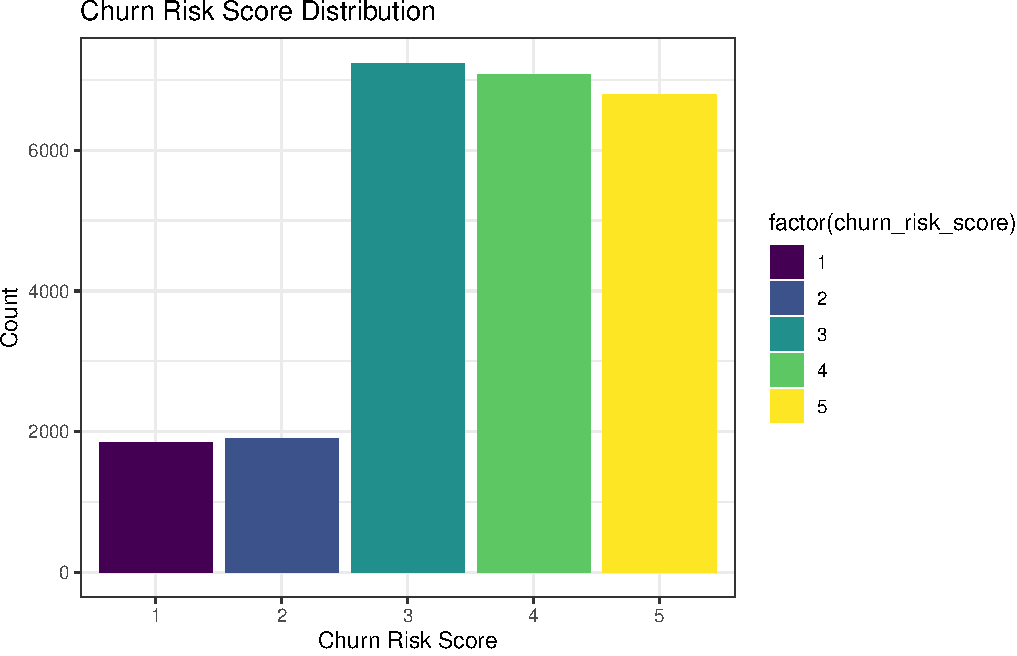
\includegraphics{FPCP4_files/figure-pdf/unnamed-chunk-20-1.pdf}
\end{center}

\begin{center}
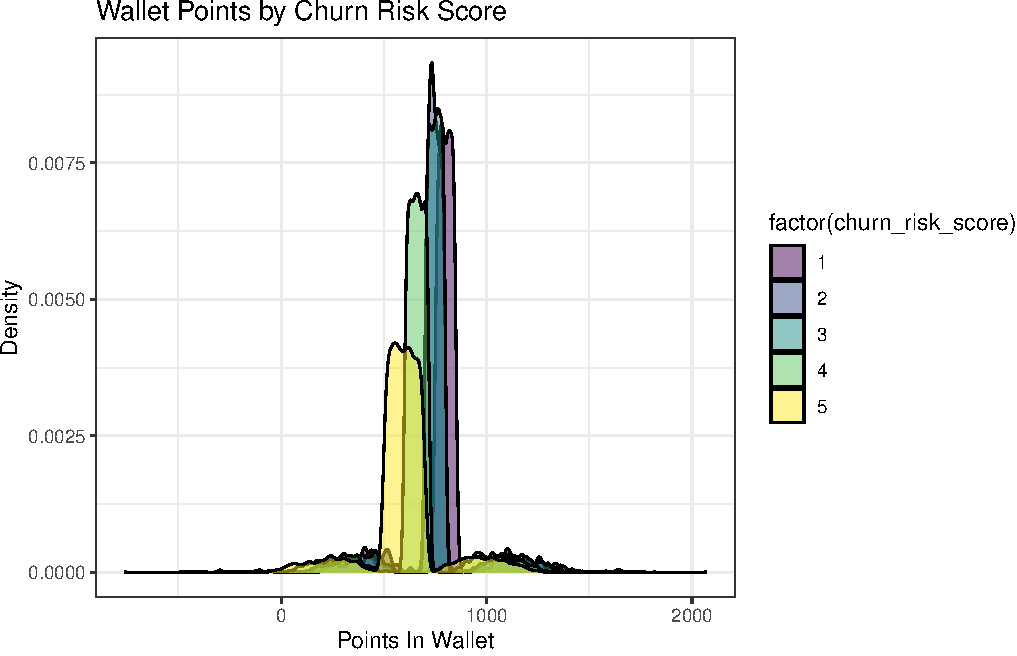
\includegraphics{FPCP4_files/figure-pdf/unnamed-chunk-21-1.pdf}
\end{center}

\begin{center}
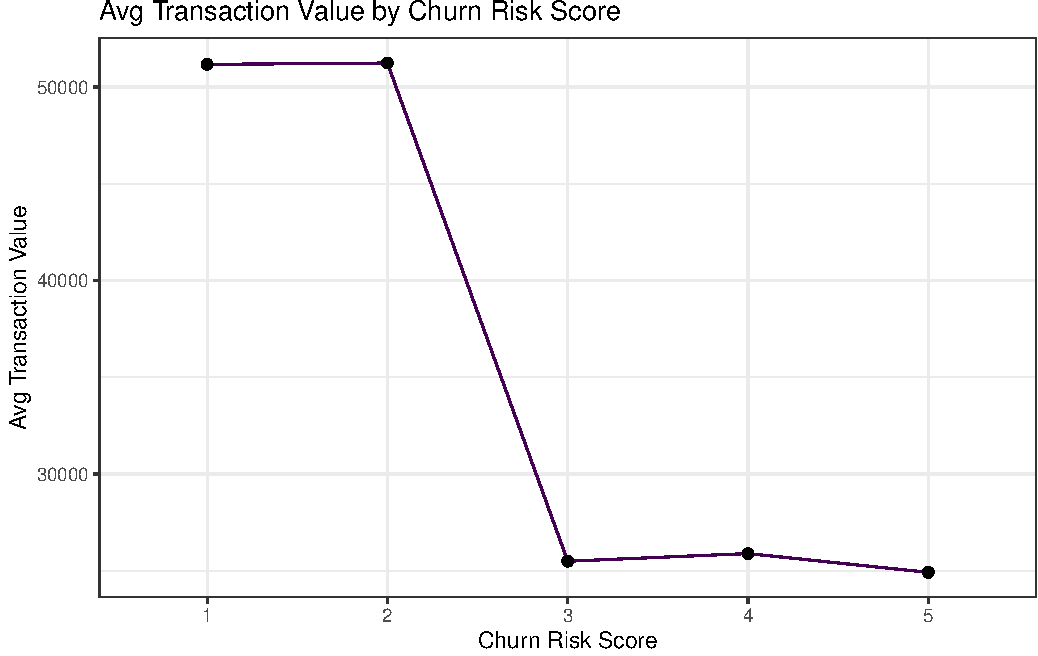
\includegraphics{FPCP4_files/figure-pdf/unnamed-chunk-22-1.pdf}
\end{center}

\begin{center}
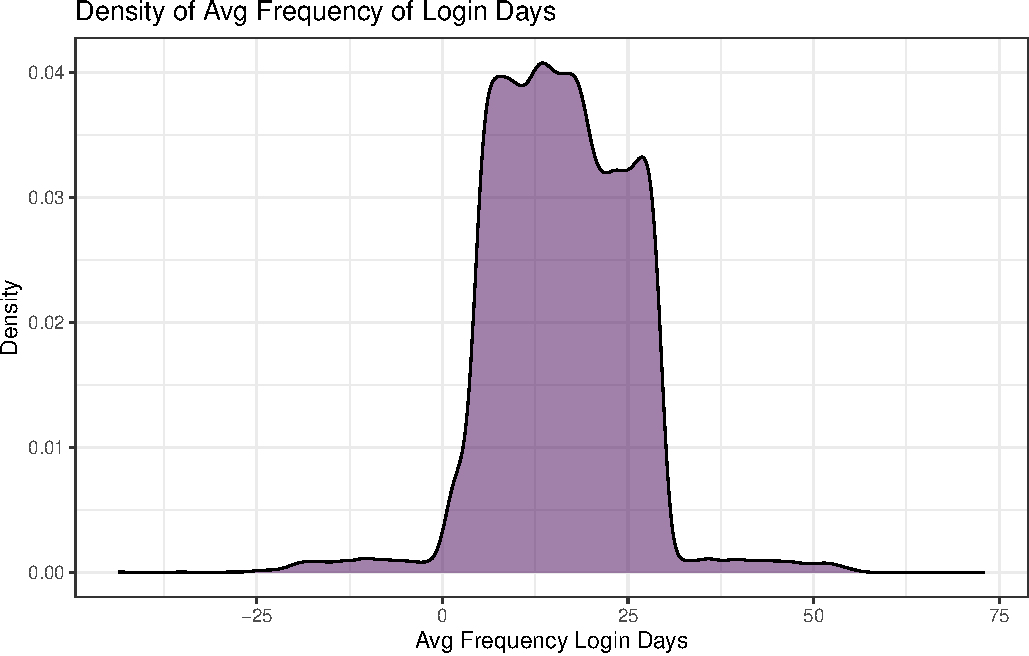
\includegraphics{FPCP4_files/figure-pdf/unnamed-chunk-23-1.pdf}
\end{center}

\begin{center}
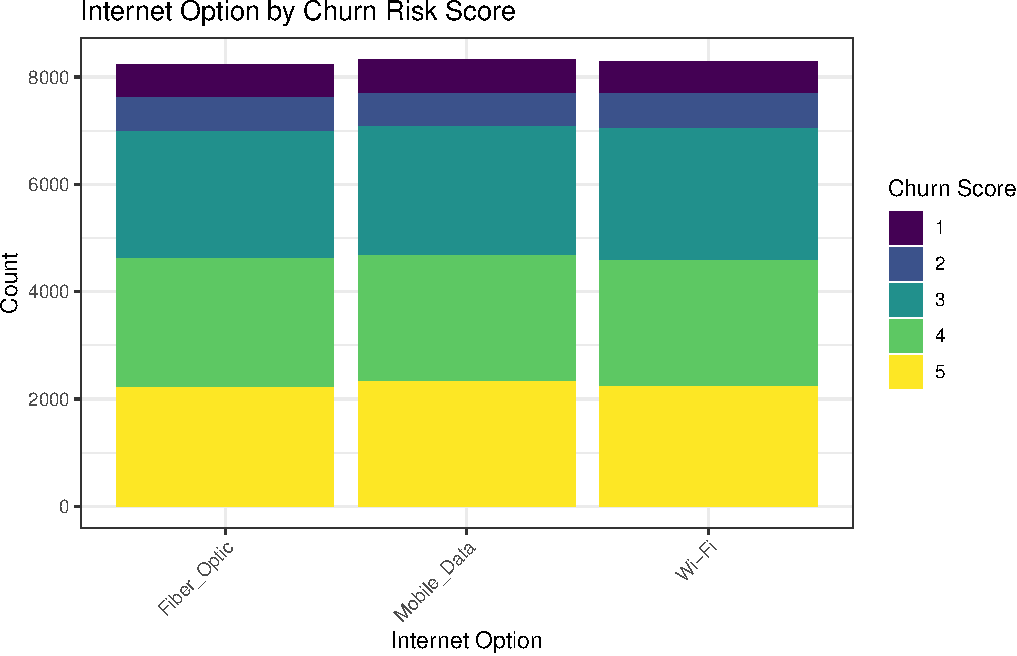
\includegraphics{FPCP4_files/figure-pdf/unnamed-chunk-24-1.pdf}
\end{center}

\begin{center}
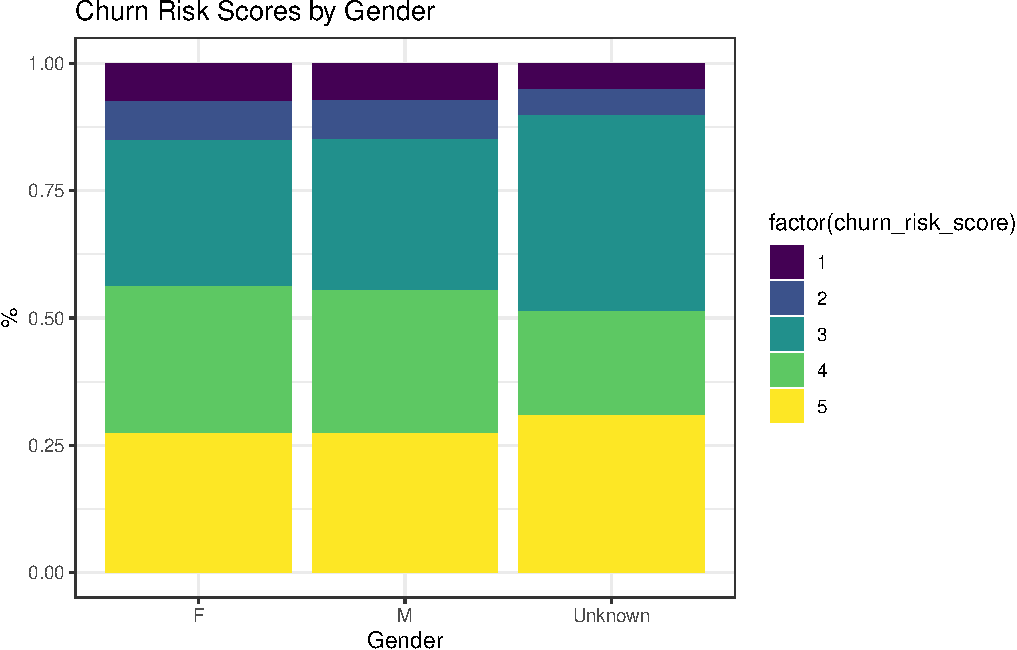
\includegraphics{FPCP4_files/figure-pdf/unnamed-chunk-25-1.pdf}
\end{center}

\begin{center}
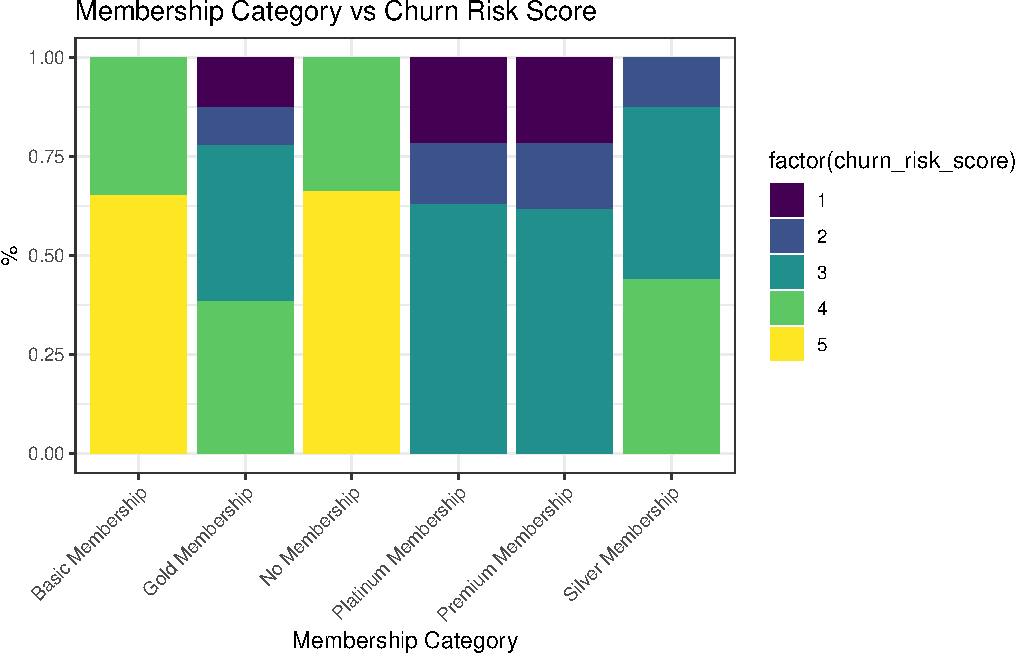
\includegraphics{FPCP4_files/figure-pdf/unnamed-chunk-26-1.pdf}
\end{center}

\begin{center}
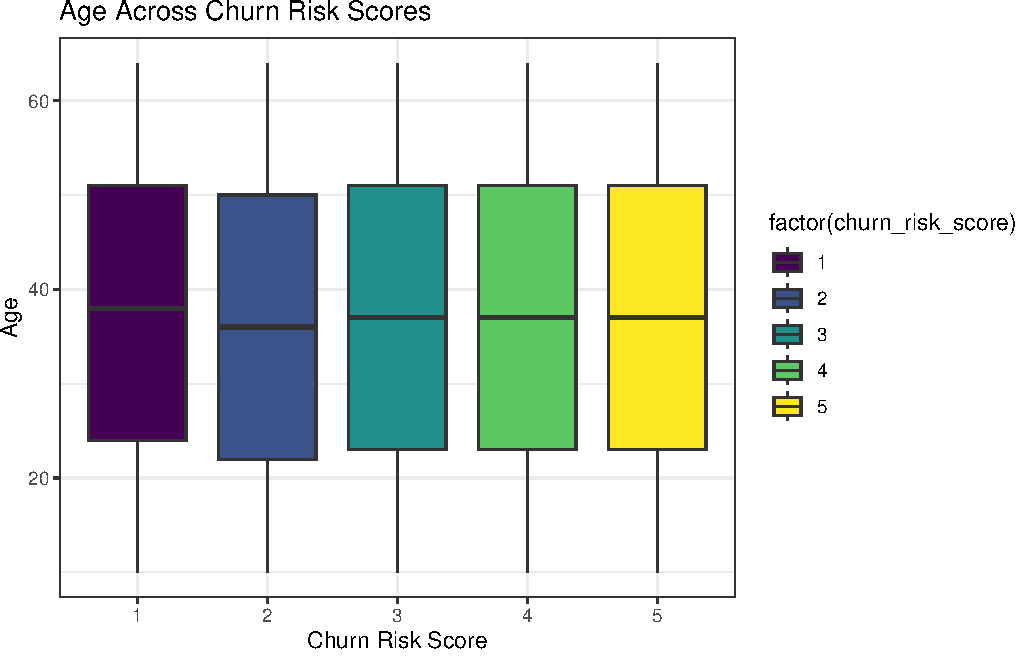
\includegraphics{FPCP4_files/figure-pdf/unnamed-chunk-27-1.pdf}
\end{center}

\begin{center}
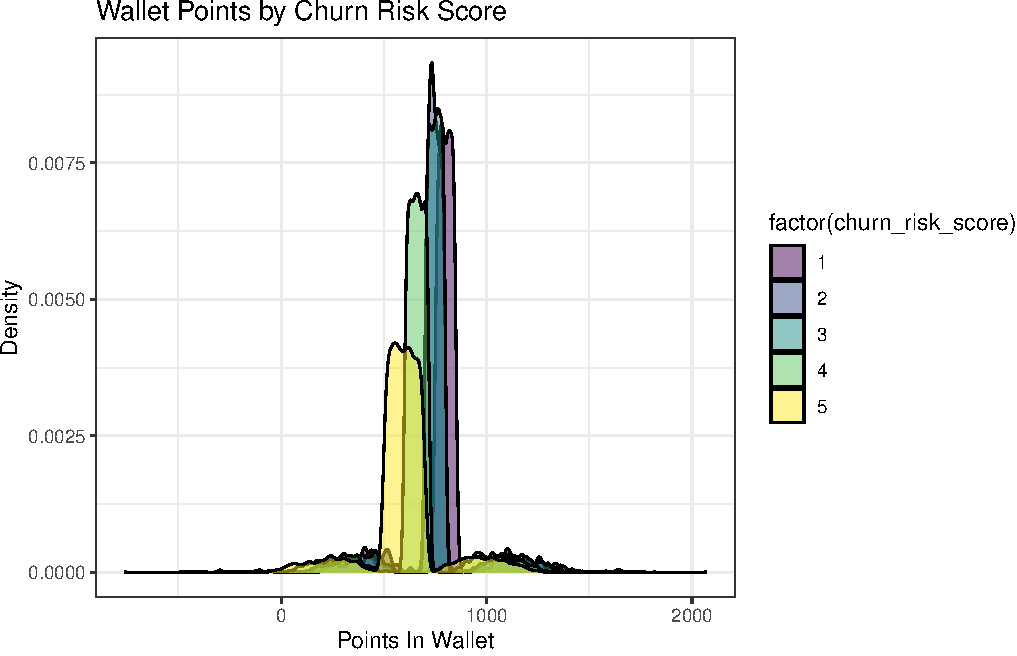
\includegraphics{FPCP4_files/figure-pdf/unnamed-chunk-28-1.pdf}
\end{center}

\begin{center}
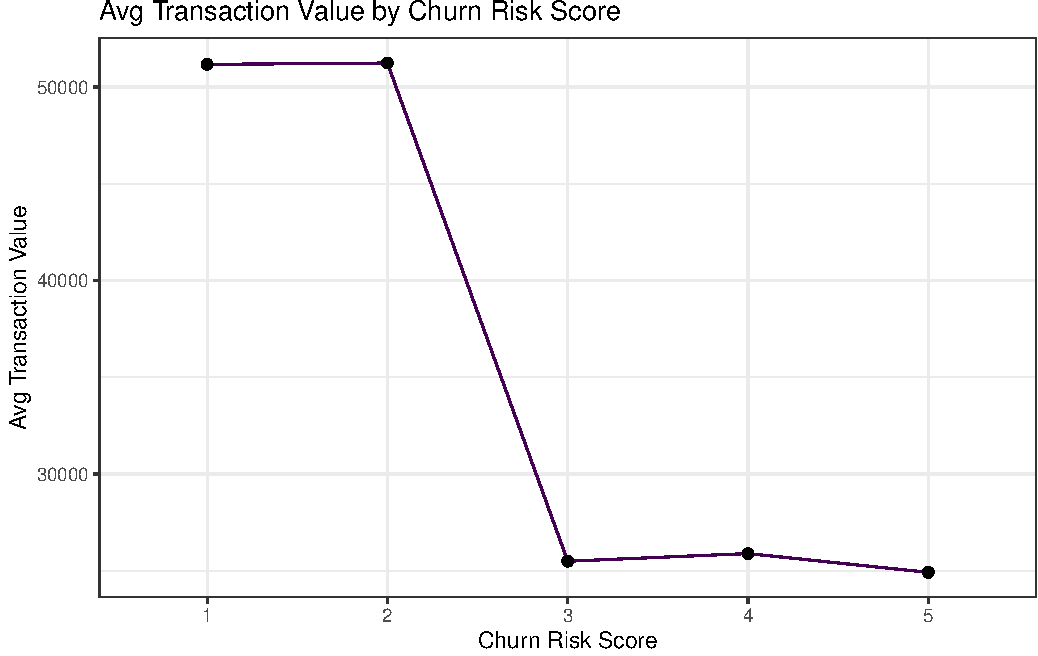
\includegraphics{FPCP4_files/figure-pdf/unnamed-chunk-29-1.pdf}
\end{center}

\begin{center}
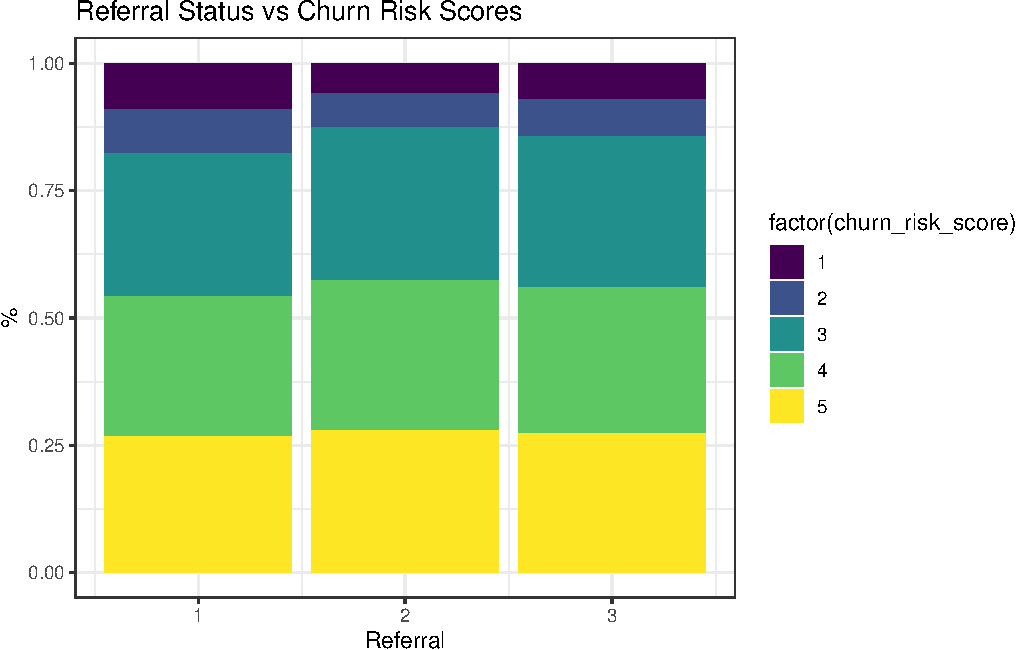
\includegraphics{FPCP4_files/figure-pdf/unnamed-chunk-30-1.pdf}
\end{center}




\end{document}
